\documentclass[titlepage]{article}
\usepackage[utf8]{inputenc}
\usepackage{hyperref}
\usepackage{float}
\restylefloat{figure}
\usepackage{color}
\definecolor{pink}{RGB}{255,102,204}
\definecolor{red}{RGB}{ 255, 51, 0}
\definecolor{orange}{RGB}{ 255, 192,0}
\definecolor{yellow}{RGB}{ 255, 255, 0}
\definecolor{green}{RGB}{ 0,176,80}
\definecolor{lgreen}{RGB}{ 146,208,80}
\definecolor{dblue}{RGB}{ 0,32,96}
\definecolor{lblue}{RGB}{ 79,129,189}

\newcommand{\pink}{\textcolor{pink}}
\newcommand{\red}{\textcolor{red}}
\newcommand{\orange}{\textcolor{orange}}
\newcommand{\yellow}{\textcolor{yellow}}
\newcommand{\green}{\textcolor{green}}
\newcommand{\lgreen}{\textcolor{lgreen}}
\newcommand{\dblue}{\textcolor{dblue}}
\newcommand{\lblue}{\textcolor{lblue}}
\usepackage{subcaption}
\usepackage{amsmath}
\usepackage{amssymb}
\usepackage{minted}
\usepackage{graphicx}
\DeclareGraphicsExtensions{.eps}
\usepackage{fancyhdr}
\pagestyle{fancy}
\lhead{Fractals and the Beauty of Nature}
\author{Chanthosh Sivanandam \\ Erik Andersen \\ Henrik Flindt }
\title{Fractals and the Beauty of Nature \\ DM550 - Fall Project 2017}
\begin{document}
\maketitle
\section{Introduction}
While the description of a tree, triangle or a leaf is easily communicated among humans, as most humans share a common cultural understanding challenges arise when trying to convey the same idea to a computer. The task assigned in DM500 requests that a script be written which can draw different figures based upon the Fractal Description Language (FDL) in the programming language, Python, by using the Turtle module. The assignment is separated into several obligatory tasks, divided into two sections; “Fractals and the Beauty of Nature” and “Fractal Description Language.”

\section{Understanding recursion}
As an illustrative explanation of recursions, a binary-tree of a depth of four, as seen in figure XX . The rule for the binary-tree is written as FLXRXLB, with F indicating a forward movement, B for a backward movement, and R and L as a right or left turn respectively. Each X indicates where each iteration (i.e. depth) would insert the rule. Table \ref{table:binary}  shows the four iterations from depth one to four. 
\begin{table}[H]
\centering
\caption{Rules for the binary tree}
\label{table:binary}
\begin{tabular}{lllll}
  \textbf{Depth} & \textbf{Rule}\\
  One   & F L R L B \\
  Two   & F L F L R L B R F L R L B L B\\
  Three &F L F L F L R L B R F L R L B \\
        & L R F B L F L R L B R F L R L  \\
  &B L B L B\\
  Four  & F L F L F L F L R L B R F L R\\
   & L B L B,R F L F L R L B R F L\\
   & R L B L B L B R F L F L F L R\\
   & L B R F L R L B L B R F L F L\\
   & R L B R F L R L B L B L B L B\\
  \end{tabular}
\end{table}
It should be noted that in the assignment, specifications for scaling of the length are included, but they have been removed from this example for a simple and smooth explanation. The colors in figure XX indicate the succession of when a line is drawn. It must be stressed that the colors do not show iterations, but first passed line in a given direction, so if two or more iterations results in a line being drawn twice, only the first passing line is drawn in the figure. The colour coded FDL for a binary-thee of depth 4 is:
\pink{F} L F L F L F L R L B R F L R L B L B,R F L F L R L B R F L R L B L B L B R F L F L F L R L B R F L R L B L B R F L F L R L B R F L R L B L B L B L B

\section{Utilizing FDL in the assignment}
The difference between one binary-tree of depth four and one binary-tree of depth 100 is only the length of the FDL and subsequent size of the tree, but the main mechanism remains unchanged.  The same mechanism would by modifying the rule, the amount of turns available, and the angle of the turns would be able to draw any figure which is shown with the Sierpinski Triangle and fern.  In this assignment additional parts have been added to the FDL mechanism that are not related to drawing lines in the Python-Turtle program, but are designed to reduce the time drawing the figure. These extra lines would in the context of the binary-tree in figure XX  as an example enable the FDL reader to jump from the end of the red line directly to the start of the orange, the end of the yellow to jump to the green line and so forth. These jumps would either be by moving the Turtle-drawer directly or by cloning the drawing instance of Turtle to the needed point. 

\section{Trial and error}
While the final product shows a fully functional FDL readers with extra functions, minor errors in the FDL rule written would sometimes result in rather interesting figures. Figure XX  show a first attempt at a fern. While this is not a ideal fern, there are several signs that the underling FDL rule are on track since there are recursions in the structure and the bend is present. \par
The first attempt took depth as a value that was transmuted in to a length that the tree and branches should cover. (In context of figure XX  this would be the length of the pink line.) 
While this in theory would work, the math needed to ensure that the scaling would result in a tree with the correct length (len) at any given depth (x) were not found. (See figure XX  for an impression of one of the failed implementations.) The main problem were a continuous mismatch between requested depth and the printed depth of the binary-tree. \par
The problem was overcome by adding depth as the secondary input factor in the definition of the object tree. (See figure XX)  Length were calculated based on the request in the assignment that a tree of the depth 10 should have the length 100. The depth value x now functioned as the iteration counter while length were scaled accordingly to the branch.\par  
The initial attempt at drawing a fern ran in to some problems in regards to hardware limitations. While the correctness and cleanliness of the code was unquestionable, the algorithm consumed incredible amounts of ram due to several factors. One of the factors was the tremendous amounts of recursive calls. An explanation hereof is, that every time a function is called in python, the interpreter allocates memory in order to store the variables in that scope. Calling a function recursively prohibits the interpreter from freeing the allocated memory from the stack until the final function has returned its value. Furthermore, and perhaps even more malignant in terms of eating ram, was the fact that the implementation made a clone of the instance of the turtle class every time there was a new branch. While this made some clean and beautiful code, an instance of the turtle class takes up a lot of memory. Some tests showed that running the algorithm for about five to ten minutes would easily take up 30 GB of ram. On the other hand, if depth and segments where kept to a minimum, the algorithm would present a nice looking fern, yet somewhat scrawny.

\section{Binary-Tree}
A simple binary-tree algorithm were written\footnote{The source code for this part of the project can be found in the file \href{https://github.com/ErikAndersen81/DM550-FractalProject/blob/master/Working_binary_tree.py}{binary-tree.py}}, which was developed to have an option to select depth. Each time a value was calculated print statements were added for that value to ensure that troubleshooting were more easily done.  A safeguard were added to the input value x to ensure that depth would be an integer, which then would be passed down through the code. The safeguard checked for strings, and force exits if one is found. Subsequently, it rounds floats and converts them to integers. (See figure XX )

Following Turtle is imported and a few definitions of Turtle functions are written. 

Minor print statements and some modifications form the Turtle package were added for aesthetics reasons and to ensure a proper user experience.  Finally the scaffolding was removed. 
\section{Sierpinski Triangle}
Initially, implementation of the Sierpinski triangle was build upon the idea of placing inverted triangles inside other triangles. It turned out to be a tad complicated, but it yielded some rather interesting results, which can be seen here:
\begin{figure}[H]
  \centering
  \begin{subfigure}[b]{0.4\textwidth}
    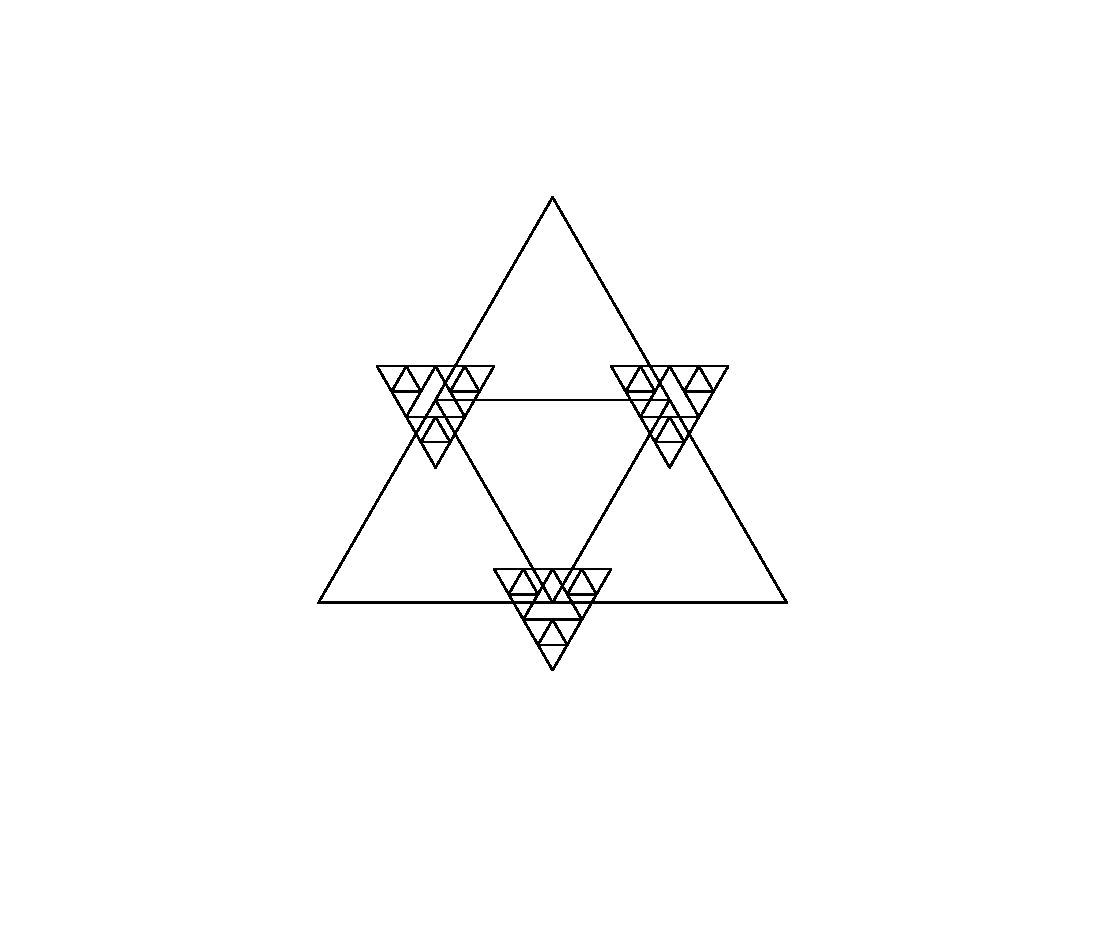
\includegraphics[width=\textwidth]{wrongtriangle}
    \caption{An unsuccessful attempt}
  \end{subfigure}
  \begin{subfigure}[b]{0.5\textwidth}
    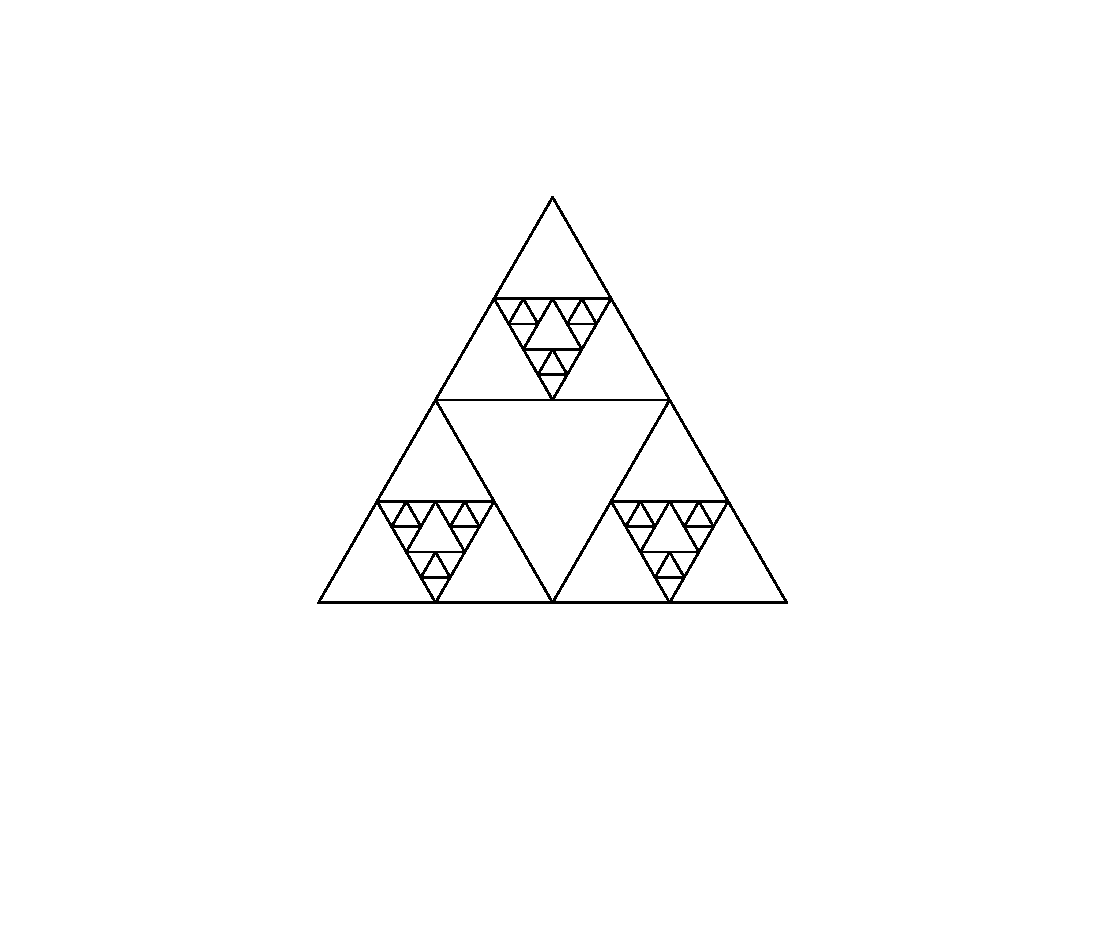
\includegraphics[width=\textwidth]{wrongtriangle2}
    \caption{Another unsuccessful attempt}
  \end{subfigure}
\end{figure}
After meddling around for some time, a decision was made to try the approach suggested in the project description. A successful algorithm that gave the expected result was then rapidly developed.
\begin{figure}[H]
  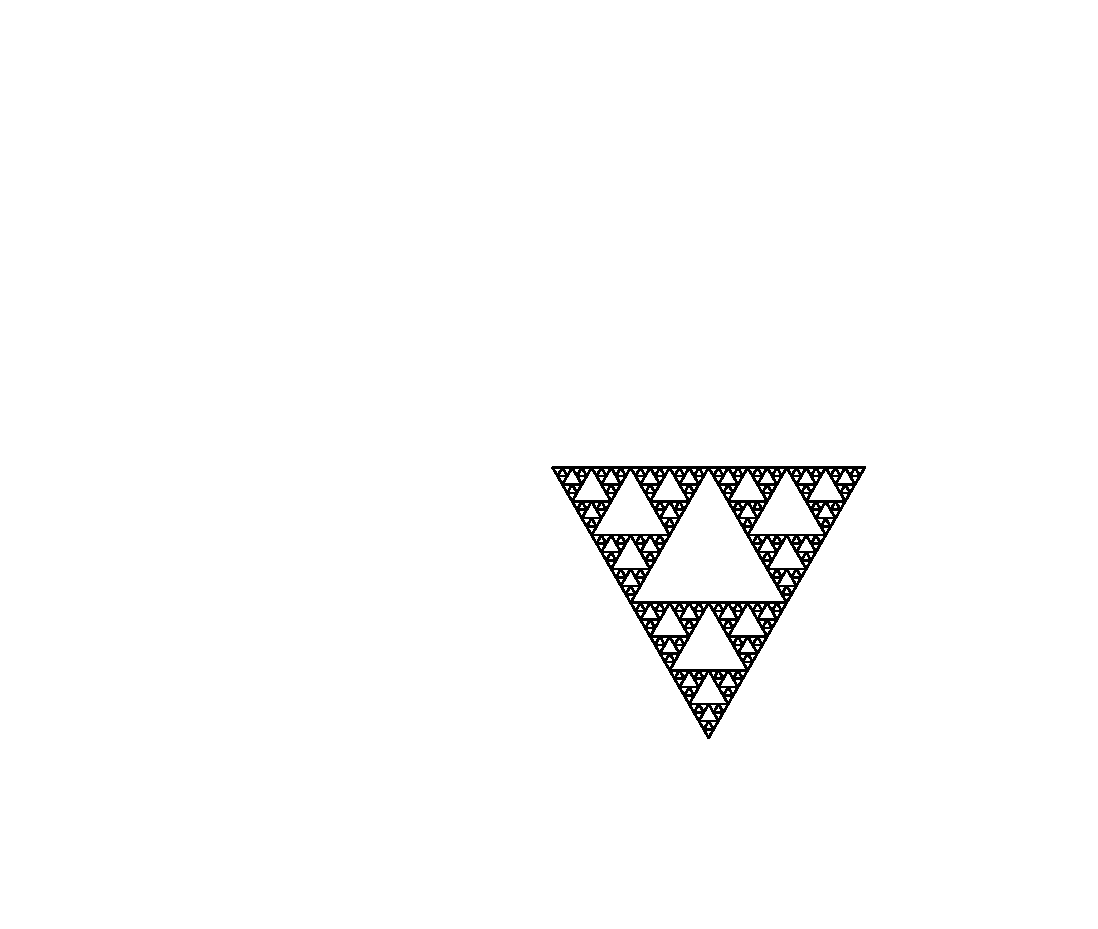
\includegraphics[width=0.6\textwidth]{triangle}
  \caption{Sierpinski triangle with 5 subdivisions.}
\end{figure}
Revisiting the initial code, the faultiness of its algorithm became apparent and hence could be corrected. The effectiveness of this new code compared to the approach recommended in the project description is due to the lack of redundant drawing. \par We used an iterative development process, meaning we started out by making a small piece of the code work in one iteration. Through testing, trial and error the goal of the iterative step was reached and we then carried on with the next step, where more code was implemented and tested. After several steps, we realized that our approach was overly complicated, so we started again from scratch. This time we did not care for optimization of the algorithm, and we solely focused on correctness.\footnote{The source code for this part of the project can be found in the file \href{https://github.com/ErikAndersen81/DM550-FractalProject/blob/master/sierpinsky-triangle.py}{sierpinsky-triangle.py}}
\begin{figure}[H]
  \centering
  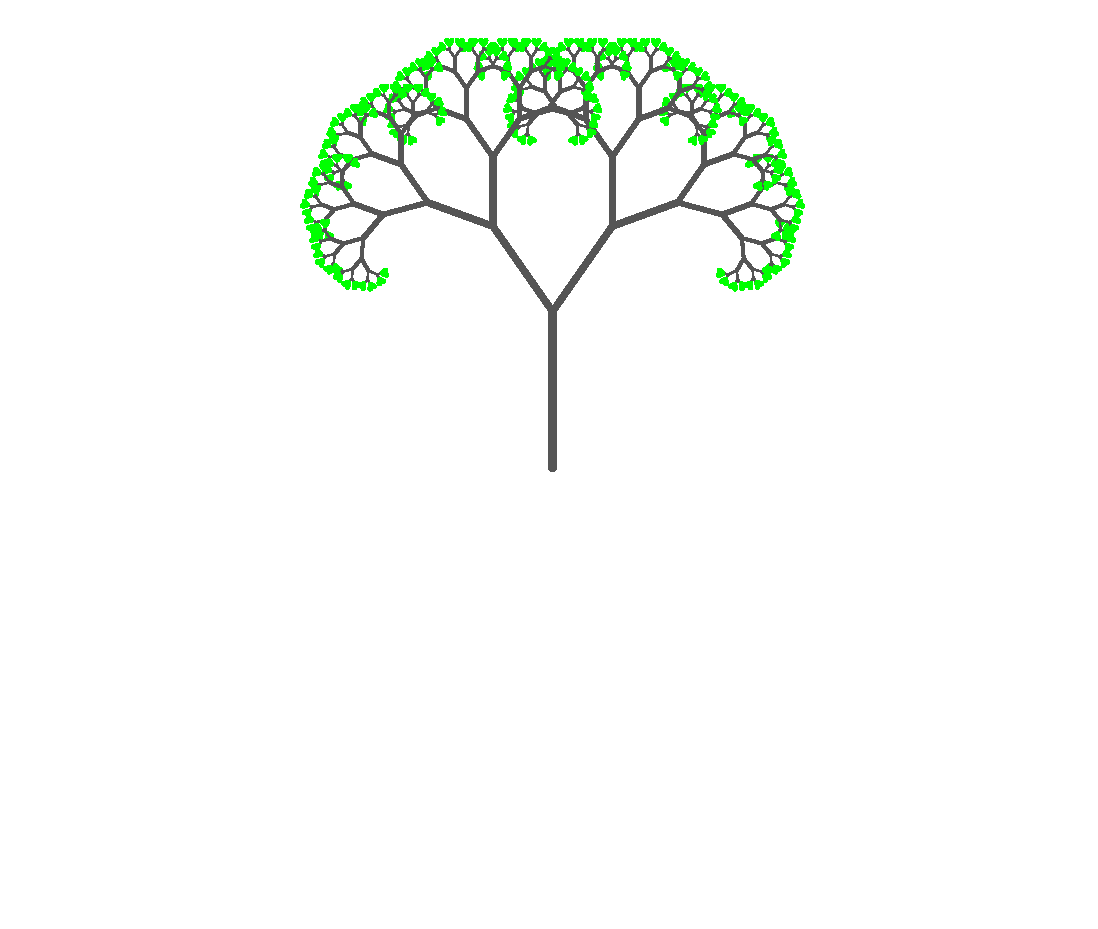
\includegraphics{bintree}
  \caption{Binary tree}
\end{figure}
\section{Binary three}
\subsection{Specification and design}
We began by trying to define a function with two parameters (size, step)
\section{FDL-Parser}
Since the fdl-file is to be read by an instance of the turtle module's Turtle class, it was decided to make a subclass of it called SmartTurtle. This class should be able to read a fdl-file, and execute he commands, giving a reasonable result. Through analysis of several fdl-files, a decision as to which attributes the SmartTurtle class should implement could be made. Thus, an instance of the SmartTurtle should have a start attribute containing a command, a length, a depth, a dictionary of rules, and one of commands which could be called with appropriate arguments. The rules should be unfolded according to the depth of the smartturtle, so a unfolded attribute would be convenient. This attribute would initially be an empty string, but when the user of the SmartTurtle class would want to execute the commands in the fdl-file loaded, a function to unfold the rules list and store them as a string in the unfolded attribute, will be required. This functionality is implemented in SmartTurtle's step function.
Since the fdl-file is to be read by an instance of the turtle module's Turtle class, it was decided to make a subclass of it called SmartTurtle. This class should be able to read a fdl-file, and execute he commands, giving a reasonable result. 
Since the instructions in the fdl file is supposed to be executed, Python's dictionary was deemed to be an appropriate data structure. The parser basically just reads through each line of the file, recognizing keywords, like \textit{start}, \textit{rule} and the like. The keywords are then used as look-ups in the dictionary yielding a string containing arguments, list of rules, or a float or int, depending on the type of keyword. 
\end{document}
